\title{A Note on the Chorales}
\author{Hugh Zabriskie}
\documentclass[12pt]{article}
\usepackage{basecommon}
\usepackage{url}
\usepackage{tikz}
\urldef{\JSBChorales}\url{https://archive.ics.uci.edu/ml/datasets/Bach+Choral+Harmony}
\tikzset{
  treenode/.style = {shape=rectangle, rounded corners,
                     draw, align=center,
                     top color=white, bottom color=blue!20},
  root/.style     = {treenode, font=\Large, bottom color=red!30},
  env/.style      = {treenode},
  result/.style	={treenode, font=\Large, top color=blue!20, bottom color=blue!20}
}
\begin{document}
\maketitle


\section{The task and background}

The task is to compose 4-part chorales in the style of J.S. Bach given a 1-part melody. Bach composed over 300 harmonization of chorale melodies, and this corpus is used today for a variety of musicianship exercises, and in particular the composition of 4-voice counterpoint. The chorales are popular as a harmonization exercise for several reasons. Firstly, the sheer number of them is attractive to both musicians and computer scientists alike, and it is rare in music to find such a large collection of similarly structured compositions. Secondly, Bach's harmonizations exemplify many of the key properties of classical Western music, such as voice leading and cadential movement, and as such are thought to be excellent studies in Classical theory. And third, Bach broke as many as rules as he seemed to establish when composing these harmonizations, and these "irregularities" are what make the chorales interesting as compositions in their own right, rather than simply being academic exercises in counterpoint. \\

Recent work with the chorales has been based on a dataset named "JSB Chorales", which was generated by Allan \& Williams (2005), available at: \JSBChorales. Confusingly, there are two versions of the data. Version 1 is much smaller, only covering 60 chorales with a total of 5665 events, and provides information about the pitch classes, beat strength, bass note, and chord symbols for each event. Greff \& Schmidhuber (2015) used Version 1 to learn next-step prediction based on sequences of binary vectors, where each vector describes the pitch classes (i.e. 'C', 'C$\sharp$', 'D', etc.) present at some time step of a chorale. Radicioni \& Esposito (2010) also used Version 1 of the chorales to build BREVE, a system for chord labelling that mapped a collection of pitch classes to a chord symbol, and which they showed to be highly accurate.\\

The second version of JSB chorales consisted of 386 chorales stored as MIDI files and sampled once per beat, so that each chorale is represented as a sequence of beat-long time frames. Boulanger-Lewandowski et. al. (2012) used this version of the dataset, along with multiple other corpuses, to train several models on the task of music generation and to model temporal dependencies within polyphonic music (i.e. how distant musical events can be related). Each MIDI file was converted into a similar sequence of binary vectors, where each vector contained a list of MIDI numbers representing the notes that occurred at a specific time step. Liu (2014) also used the second version to "re-construct" chorales with an RNN by feeding chorales during training and then providing the beginning notes of each chorale in the test set as initial input to see if the rest of the composition could be re-composed - melody and harmony together.\\

Note that none of the recent papers described above work on the task of harmonization, but some work on related tasks such as chord identification and, more generally, music generation. Version 1 of the data does not identify the melody, only the pitch classes present and their corresponding chord symbol, making the task of harmonization impossible to learn on this data alone. Version 2, moreover, does not identify specific voices (i.e. it is unclear which voice belongs to the alto versus to the tenor) and the creators of the dataset only did a mediocre job at simplifying each chorales into a series of representative chords at each step. The data used in this paper improves upon this version by more carefully "quantizing" the chorales into sequences of beat-long time frames while also identifying each note with one of the 4 voices. The most well-known attempts at chorale harmonization in the last decade did not use neural networks in their models. Allan \& Williams (2005) used Hidden Markov Models with reasonable success and Buys \& Merwe (2012) used weighted finite-state transducers (WFST) and had results "competitive" with Allan \& Williams.  \\ 

In short, the original task of harmonizing chorales, has not been approached as effectively or thoughtfully, in the opinion of the author, since the HARMONET system was published by Hild, Feulner, and Menzel in 1992. HARMONET completes the task of harmonization using 3 neural nets where the output of one is fed as input to the next. The first network selects a "harmonic skeleton" that outlines the harmonies for the entire chorale, the second net selects the alto and tenor voices, and the final net adds rhythmic ornamentation (i.e. passing tones) to better model the rhythmic patterns in Bach's original harmonizations. In all recent papers, rhythmic complexity has been entirely factored out to focus on other aspects of the music. While HARMONET was not evaluated qualitatively, the chorales it produced were judged to be "on the level of an improvising organist" - a rather glowing review. Moreover, it was only trained on 40 chorales (split evenly between major and minor keys) rather than the entire collection of chorales. Therefore, in many ways HARMONET provides a strong model for approaching the task of harmonization while also leaving room for improvement. since neural networks and the field of machine learning generally have developed significantly since this model was published.

\subsection{The task computationally}

Mathematically, let's define the task more concretely. The algorithm should take as input the chorale, represented a sequence of notes, and it should output a corresponding sequence of 3-voice chords that represent the alto, tenor, and bass voices. Following the approach of HARMONET, the task is divided into 3 steps:
\begin{enumerate}
\item Creation of a harmonic skeleton in the form of Roman numeral analysis. This also implies a bass line.
\item The selection of the alto voice.
\item The selection of the tenor voice.
\end{enumerate}
We assume that we are given a sequence of symbols from a vocabulary $V$. That sequence represents an entire chorale.
$$x_1, x_2, x_3, \ldots \quad x_i \in V$$
Each symbol $x_i$ describes a set of features about the melody at time $i$. Those features include, but need not be limited to:
\begin{itemize}
\item The pitch of the melody at time $i$. Optionally, pitches that comes directly before or after it as well ($i-1$, $i+1$).
\item The beat strength, to add metrical context (i.e. is it on a downbeat?).
\item Whether a cadence occurs at time $i$, represented by a fermata.
\item Chorale-specific information, such as the key signature and time signature.
\end{itemize}

\noin Let's say we have $m$ data points with $n$ features, and $Y$ output classes.
\begin{itemize}
\item $\boldX \in V^{m \times n}$ is our input data
\item $\boldY \in Y^m$ is our output data
\end{itemize}

\subsection{Recurrent model}

Another potential source of information in a recurrent model is the harmony chosen in the previous computation for time $i-1$. Many papers have suggested the importance of knowing previous chosen harmonies in predicting subsequent harmonies, which is in line with the musical conception of harmony as a \textit{progression}. Often in Western music, and always within the chorales, a chord or harmony is viewed within the context of its surrounding harmonies, a component in a progression. We treat the importance of the preceding harmonies as a hypothesis. And this hypothesis is tested by an "Oracle experiment" that examines whether a baseline model improves when trained with the knowledge of the harmony that directly precedes it.    


\section{Baseline model}

The baseline model for this task is defined as a generic, non-recurrent neural network that learns to map each time frame of the melody to an acceptable harmonization. For the subtask of Roman numeral analysis, the input data $\boldX$ contains over 20,000 data points, split into training and testing sets, with a vocabulary size of 221. The output data $\boldY$ has 57 classes, each describing a specific harmony within the context of a key (i.e. 'IV', 'ii7', etc.). The set of output harmonies was generated by running over each data point and using music21's roman numeral analysis library to determine the harmonic function. The resulting set of harmonies (i.e. 'ii7$\sharp$42', 'V6') was mapped to a smaller output space of only root and seventh chords (i.e. 'ii7', 'V'). Note that major seventh chords and dominant seventh chords were not treated differently here.

\begin{center}
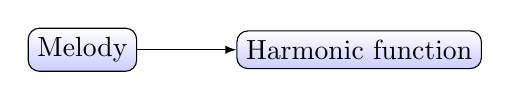
\begin{tikzpicture}
  [
    grow                    = right,
    sibling distance        = 6em,
    level distance          = 10em,
    edge from parent/.style = {draw, -latex}
  ]
  \node [env] {Melody}
    child { node [env] {Harmonic function} };
\end{tikzpicture}
\end{center}


The results from 200 epochs are shown below. The learning rate was set at $0.00001$, the vocabulary embedding size ($d$) was $100$ and the hidden layer size was $100$. 

\begin{center}
  \begin{tabular}{ c | c }
    Accuracy & Average NLL per chorale \\ \hline
    33.67\% & 98.242
  \end{tabular}
\end{center}

\subsection{Improving the baseline}

The baseline model was changed for 2 reasons: 1) to improve classification accuracy, and 2) to improve the diversity of harmonic possibilities. The task of creating a harmonic skeleton was divided into two subtasks: one in which the Roman numeral is chosen (i.e. 'I', 'iv', 'bVII') and the second in which the inversion is chosen. Note that the output of the second subtasks (the choice of inversion for each Roman numeral) implies a bass line.\\
Generation of the Roman numeral and inversion for each data point was performed using the \texttt{roman} module of music21's Python library combined with some manual correction.

\begin{center}
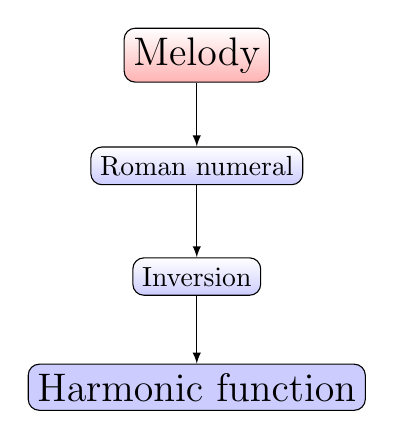
\begin{tikzpicture}
  [
    grow                    = down,
    sibling distance        = 6em,
    level distance          = 4em,
    edge from parent/.style = {draw, -latex}
  ]
  \node [root] {Melody}
    child { node [env] {Roman numeral} 
    	child { node [env] {Inversion} 
		child { node [result] {Harmonic function} }}};
\end{tikzpicture}
\end{center}

\subsection{Numeral subtask}

\begin{center}
	\begin{tabular}{ c | c | c | c }
		\textbf{Total NLL} & \textbf{Accuracy} & \textbf{Accuracy (no I)} & \textbf{Accuracy (no I, no V)} \\ \hline
		3783.590 & 36.96\% & 26.27\% & 15.21\%
	\end{tabular}
\end{center}	 

\subsection{Inversion subtask}

For the inversion subtask, training the model to classify all inversions performed poorly. This is most likely due to the sparse data on chords not in root position or 1st inversion. Choosing the root chord for virtually every example gave approximately a 55\% accuracy rate, but the model failed to classify other inversions. The inversion subtask itself could be broken into a series of smaller decisions. Several classification tests were run to determine the model's ability to identify a specific inversion among the other options. 

\begin{center}
	\begin{tabular}{ c | c | c | c | c }
	\textbf{Inversion} & \textbf{Accuracy} & \textbf{Sensitivity} & \textbf{Specificity} & \textbf{F1 Score} \\ \hline
	Root & 70.03\% & 69.13\% & 71.14\% & 0.718 \\
	\end{tabular}
\end{center}

Upon removing all examples in root inversion, the classification accuracy increased significantly, but not to a desired level. It once again overwhelmingly predicted the most frequent inversion, 1st inversion, which represents the 2nd most common inversion in the dataset.

\begin{center}
	\textbf{With root removed}
	\begin{tabular}{ c | c | c | c | c }
	\textbf{Inversion} & \textbf{Accuracy} & \textbf{Accuracy (1st inv)} & \textbf{Accuracy (not 1st inv)} & \textbf{F1 Score} \\ \hline
	All & 48.02\% & 95.51\% & 31.58\% & 0.905 \\ \hline
	1st inv & 68.20\% & 59.06\% & 75.28\% & 0.619 \\
	\end{tabular}
\end{center}

\begin{center}
	\textbf{With root and 1st inversion removed: }
	\begin{tabular}{ c | c }
	\textbf{Inversion} & \textbf{Accuracy} \\ \hline
	All & 32.88\% \\
	\end{tabular}
\end{center}

\subsection{Numeral subtask - Oracle experiment}

\begin{center}
	\begin{tabular}{ c | c | c | c }
		\textbf{Total NLL} & \textbf{Accuracy} & \textbf{Accuracy (no I)} & \textbf{Accuracy (no I, no V)} \\ \hline
		4082.023 & 32.78\% & 20.54\% & 11.73\%
	\end{tabular}
\end{center}	



\end{document}